% Event code alignment test script - Documentation - Top level
% Written by Christopher Thomas.

\documentclass[letterpaper,11pt]{report}
\usepackage[letterpaper]{geometry}
\usepackage{graphicx}
\usepackage{verbatim}
\usepackage{placeins}
\usepackage{longtable}

\geometry{nohead,footskip=0.3in,margin=0.75in}

% Force my paragraph style, darnit.
\usepackage{indentfirst}
\setlength{\parskip}{\baselineskip}

% NOTE - "\thispagestyle" is used for part and chapter beginning pages, and
% overrides \pagestyle. Redefine it to be harmless.
% NOTE - The canonical solution ("\pagenumbering{gobble}") resets the page
% counter whenever it's used.
\renewcommand{\thispagestyle}[1]{}

% Custom macros.
\newcommand{\fixme}[1]{\textbf{FIXME: #1}}

\newcommand{\figdef}[3]
{\begin{figure}[htb]
\begin{center}#1\end{center}
\caption{#2}\label{#3}\end{figure}}

\newcommand{\tabdef}[3]
{\begin{table}[hb]
\begin{center}#1\end{center}
\caption{#2}\label{#3}\end{table}}

% Document body.
\begin{document}
%
% Title page.
%
\pagestyle{empty}

\begin{center}
%
\vspace*{0.5in}
{\Huge Event Code Alignment Test Script \\ Code Reference} \\
{\footnotesize Written by Christopher Thomas -- \today.}
%
\vspace*{0.5in}\\
%
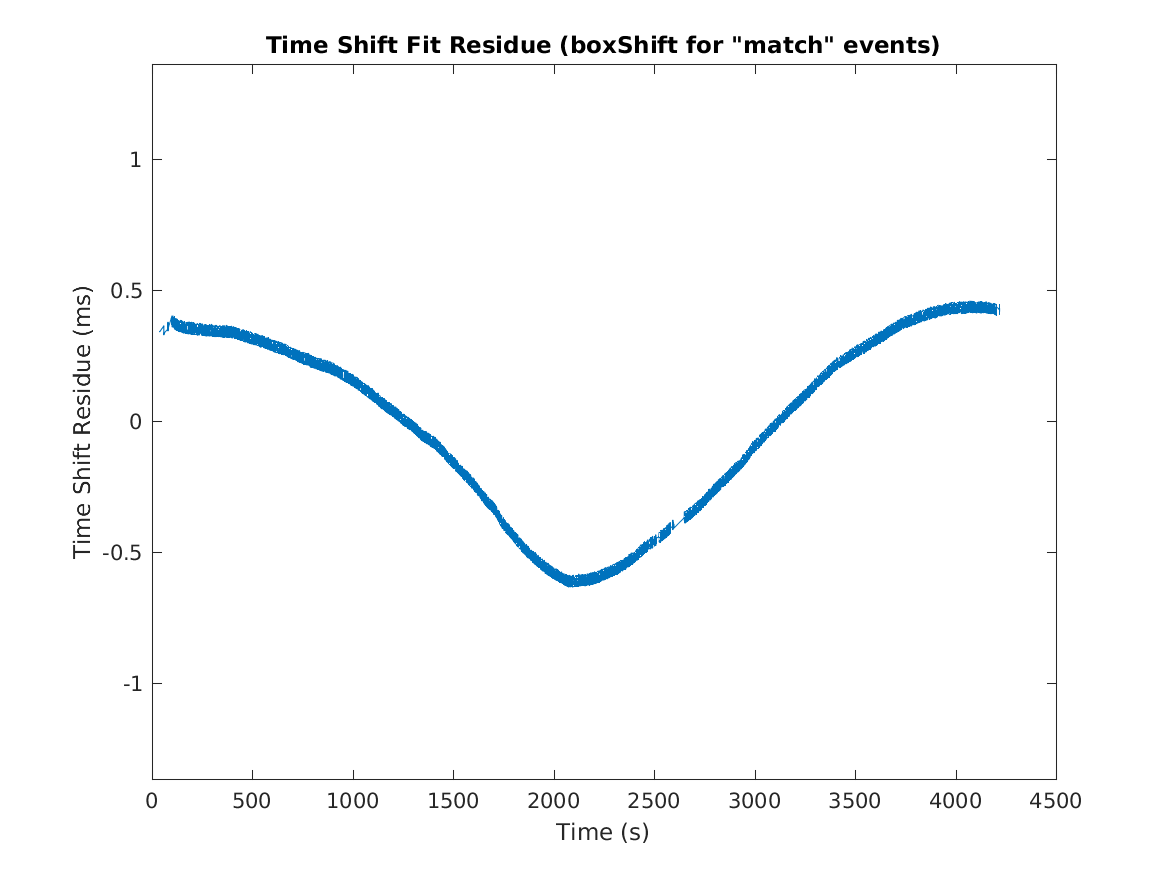
\includegraphics[width=4in]
{plots/20211018/test-boxreply-shift-match-delta-residue}
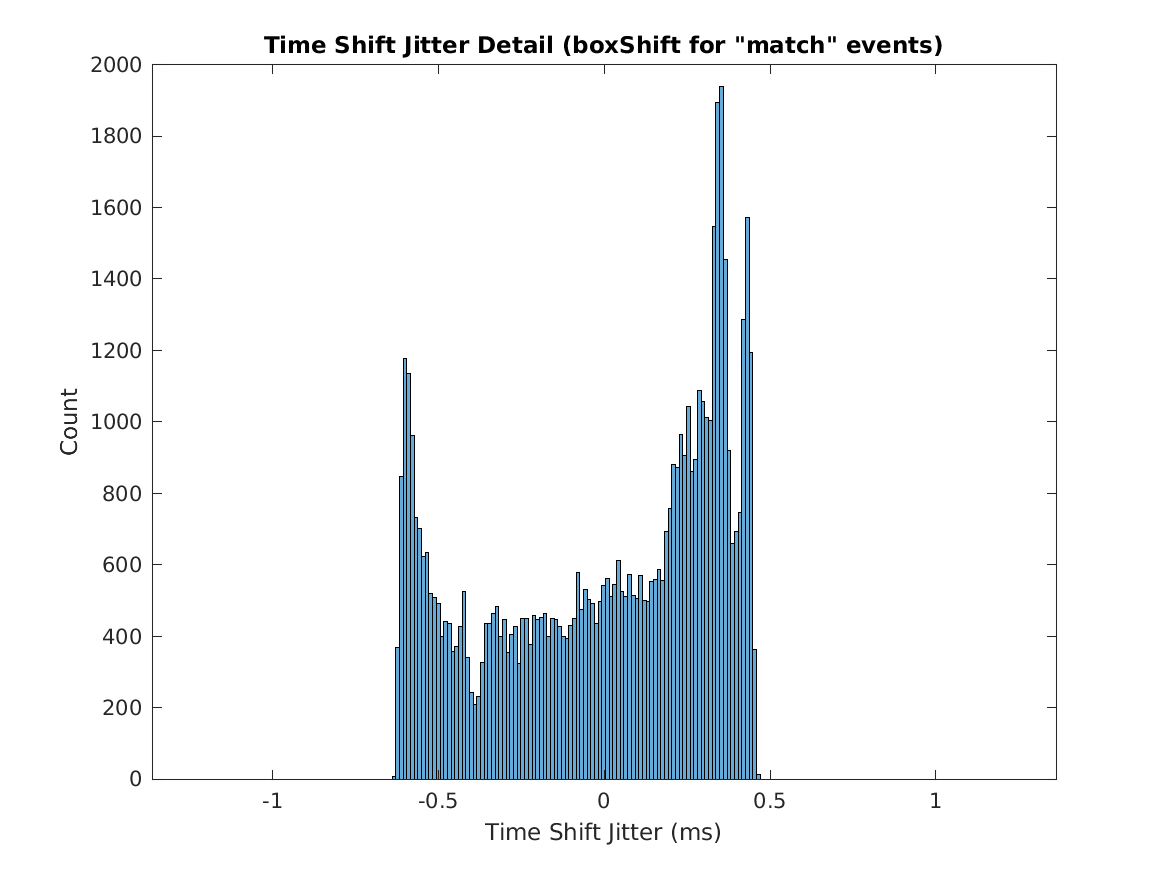
\includegraphics[width=4in]
{plots/20211018/test-boxreply-shift-match-delta-jitter-core}
%
\end{center}
%
\vfill
% FIXME - No license, as this isn't for public release yet.
%{\tiny \input{../../LICENSE.md}}
%
\clearpage
%
%
% Front matter.
%
\pagestyle{plain}
\pagenumbering{roman}
\setcounter{page}{1}
%
\tableofcontents
\clearpage
%
%
% Document parts.
%
\pagestyle{plain}
\setcounter{page}{1}
\pagenumbering{arabic}
%
\input{euscript-evcodes-readme}
\clearpage
%
\input{euscript-evcodes-dostuff}
\input{euscript-evcodes-helpers}
%
%
\end{document}

%
% This is the end of the file.
